\chapter{Overview of a DBMS}

This chapter will give a general overview of the structure of a centralized \textbf{DBMS} (\textbf{Data Base Management System}) based on the relational data model, describing its components and their respective functionalities.

\section{Architecture}

A database is a collection of homogeneous sets of data, with relationships defined among them, stored in permanent memory, and used via a DBMS.

\BoxDef{DBMS}{
A DBMS is a software that provides the following functionalities:
\begin{itemize}
    \item A language to describe the \textbf{schema} of the database (a collection of definitions that describe the data structures), restrictions on the allowed data types, and the relationships among data sets;
    \item The data structures for storage and efficient retrieval of large amounts of data;
    \item A language to guarantee secure access to the data only to authorized users;
    \item A \textbf{transactions} mechanism to protect data from HW/SW malfunctions and errors during concurrent access.
\end{itemize}
}

The architecture of a DBMS provides the following basic components:
\begin{itemize}
    \item The \textbf{Storage Engine}, which includes modules supporting:
    \begin{itemize}
        \item \textbf{Permanent Memory Manager};
        \item \textbf{Buffer Manager};
        \item \textbf{Storage Structures Manager};
        \item \textbf{Access Methods Manager};
        \item \textbf{Transaction and Recovery Manager};
        \item \textbf{Concurrency Manager}.
    \end{itemize}

    \item The \textbf{Relational Engine}, which includes modules supporting:
    \begin{itemize}
        \item \textbf{Data Definition Language};
        \item \textbf{Query Manager};
        \item \textbf{Catalog Manager}.
    \end{itemize}
\end{itemize}
In real systems the functionalities of these modules are not completely separated in different components (as in Figure \ref{fig:DBMS_schema}), but this overview can help in understanding the purpose of each of them. 

\begin{figure}[h]
    \centering
    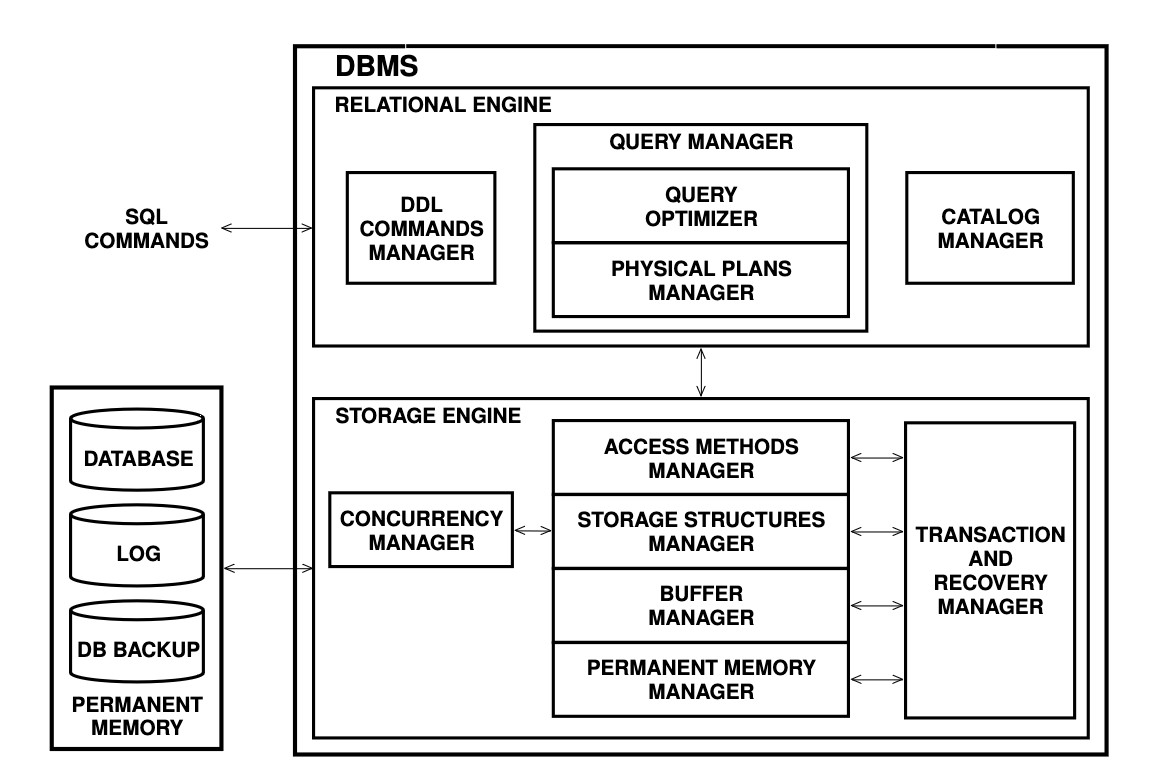
\includegraphics[width=0.75\linewidth]{img/DBMS schema.png}
    \caption{The architecture of a DBMS.}
    \label{fig:DBMS_schema}
\end{figure}

\subsection{Permanent Memory Manager}

The PMM manages page allocation and deallocation on disk storage. It hides the disk characteristics and the operating system, as it provides an abstraction of the memory as a a set of databases, each consisting of a set of logical files of \textbf{physical pages} (or blocks) of fixed size. The physical pages of a file are numbered consecutively starting from 0, and their number can grow dynamically with the only limitation being the available space in the permanent memory. Each collection of records (table or index) of a database is stored in a logical file, which can also be realized as an actual separate file of the operating system or as part of a file in which the database is stored.

Once a physical page is transferred to main memory, it is called a \textbf{page}, and it is represented with a specific, complex structure.

\subsection{Buffer Manager}

The Buffer Manager is tasked with transferring pages between temporary and permanent memory. It allows transactions to get the pages they need minimizing the number of disk accesses. In general, the performance of operations on a database depends on the number of pages transferred to temporary memory. If a big enough buffer is used, and there's a high number of access requests for a specific page, there's a high likelihood that such page will be in the buffer. Figure \ref{fig:buffermanager} illustrates the basic structure of a Buffer Manager.

\begin{figure}[h]
    \centering
    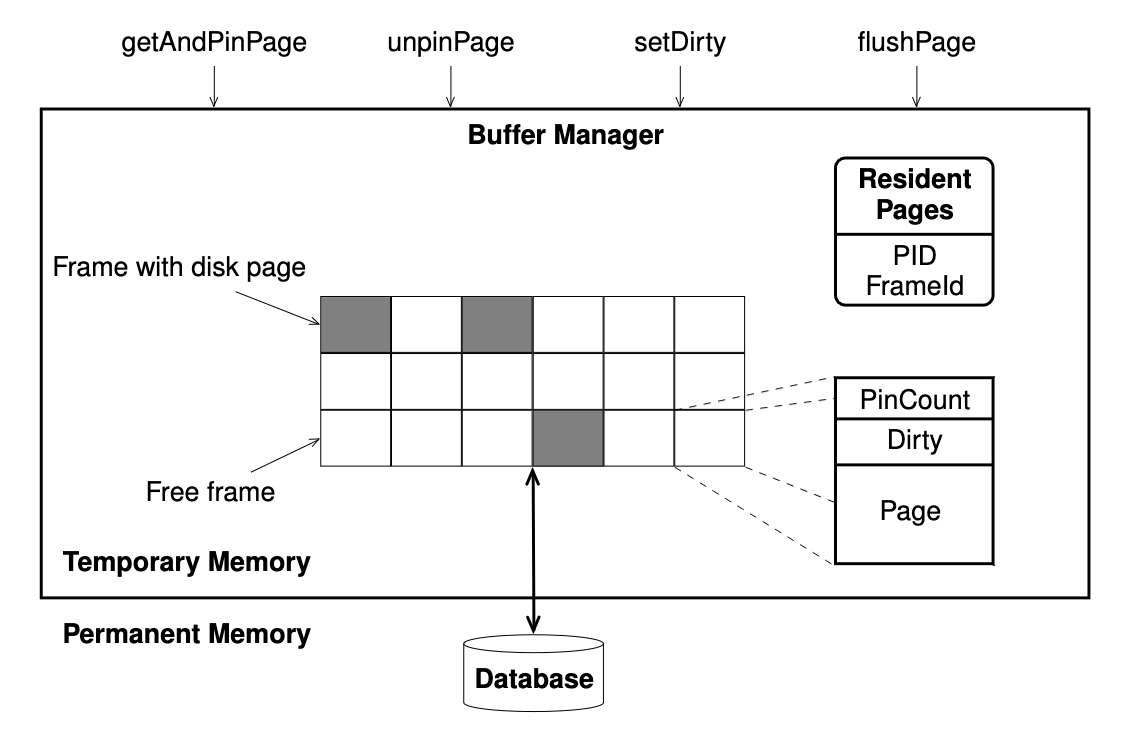
\includegraphics[width=0.5\linewidth]{img/Buffer Manager.png}
    \caption{The components of the Buffer Manager.}
    \label{fig:buffermanager}
\end{figure}

The \textbf{buffer pool} is an array of \textbf{frames}, each containing a copy of a page present in permanent memory, and some additional bookkeeping information. The pool has a fixed size, so when there are no more free frames, a page must be freed with an appropriate algorithm. Each frame stores two variables, the \textbf{pin count} and the \textbf{dirty}. The former counts the number of transactions currently using the page hosted on that frame; its value starts at 0, and increases by 1 each time it is requested, and decreases by 1 each time it is released. The latter indicates whether the page was modified since it was copied into the buffer, signaling that the modification must be reflected on disk as well. The \textbf{resident pages} table is a hash table that is used to know which page in permanent memory (identified by a PID) is stored in which frame.

A commonly used replacement policy id the \textbf{Least Recently Used} (\textbf{LRU}) policy. Once the buffer pool is full, the frame chosen to be ejected is the one that was the earliest one to be pinned. The idea is that since the page hasn't been requested for a relatively long time, it probably won't be requested any time soon. However, this policy may not always be the best: for example, in a join loop between two tables, the LRU policy may be optimal for one table, while the optimal one for the other is Most Recently Used (MRU).

\subsection{Storage Structures Manager}

The Storage Structure Manager implements databases as tables of records, representing the files of pages provided by the Permanent Memory Manager. Above the Storage Structure Manager, the unit of access is a record; below, the unit of access is a page. For this reason, the unit of costs considered for now will be a single page access (read or write), and we assume that memory operations have 0 cost, since they're so much faster than disk operations their addition to the overall cost is negligible. The most important type of file is the \textbf{heap file}, which stores records in no particular order.

A \textbf{record} is a collection of one or more \textbf{attributes}, and contains some extra information, called \textbf{record header}, needed for record management. We assume records are not larger than a page (a few KB big), and that each attribute is either separated from the others using a separator, or all attributes are stored sequentially and are indexed by using an offset. Each record is uniquely identified by a \textbf{RID}, which specifies the page and the offset the record can be found at. Sometimes this offset may be logical, i.e., it actually indicates a position on an array of actual pointers to records; this way, records can be moved around without having to externally modify their RID.

Collections of pages may be stored using different data structures. Usually, pages are stored with two alternatives. The first uses two doubly linked list, one containing free pages, the other containing full ones. The other alternative consists in a \textbf{directory}, where each entry contains a pair PID-available space. If the directory grows and cannot be stored in the header page of the file, it is organized as a linked list. For efficiency reasons, the free space existing in different spaces cannot be compacted into new free pages. If the available free space is plenty but there's no actual free pages available, it may be necessary to reorganize the database.

\section{Data Organizations}

\subsection{Heap and Sequential Organizations}

The data can be arranged either via \textbf{heap organization}, or \textbf{sequential organization}. With heap organization, every new record is added to the end of the file: insertion is easy and efficient in terms of memory used. It is ideal for situations where insertion is more common than search, or files where massive search is common. This is also the standard organization for DBMS.

With sequential organization, data is kept sorted on a \textbf{search key} $K$, picked as a single attribute of the records. This makes equality and range search on $K$ very efficient. On the other hand, insertion is more problematic, since the ordering of the records must be maintained at all times. Insertion may use a \textbf{static solution}, where each page is filled normally, and for each insertion, the record is placed at the correct spot in the ordering, moving all other records after it. A \textbf{dynamic solution} instead keeps some fraction of the total space in a page free. Once a page has filled up enough, its contents are split into new pages. This way, pages always have some extra space at the end to accommodate new insertions: when a record is added, the shifting of the records after it will only involve the ones in the same page. Alternatively, a \textbf{differential file} may be used to keep track of which changes must be applied to which pages, so that all insertions can be done all at once in a second moment.

Table \ref{tab:heap-seq-comp} shows a comparison between the two organization types. $N_{pag}(R)$ refers to the number of pages required to store the records. The \textbf{selectivity factor} $sf$ is an estimate of the fraction of pages occupied by records that satisfy the condition of a range search, and is calculated as:
\begin{equation*}
    sf = \dfrac{(k_2 - k_1)}{(k_{max} - k_{min})} \ ,
\end{equation*}
with $k_1$ and $k_2$ being the two extremes of the range, and $k_{max}$ and $k_{min}$ the highest and lowest values in the domain of the attribute.

\begin{table}[h]
\small
\centering
\SetTblrInner{rowsep=5pt}
\begin{tblr}{hlines, vlines, columns={75pt, c, m}, column{1}={50pt, c}, column{2}={50pt, c}, column{5}={50pt,c}, column{6}={50pt, c}}
        \textbf{Type} & \textbf{Memory} & \textbf{Eq. Search} ($C_s$) & \textbf{Range Search} & \textbf{Insertion} & \textbf{Deletion} \\
\hline
        \textbf{Heap} & $N_{pag}(R)$ & $\ceil{\dfrac{N_{pag}(R)}{2}}$ & $N_{pag}(R)$ & $2$ & $C_s + 1$ \\

        \textbf{Seq.} & $N_{pag}(R)$ & $\ceil{\log_2{N_{pag}(R)}}$ & $C_s - 1 + \ceil{sf \times N_{pag}(R)}$ & $C_s + 1$ $+ N_{pag}(R)$ & $C_s + 1$ \\

\end{tblr}
    \caption{Comparison between heap and sequential organization.}
    \label{tab:heap-seq-comp}
\end{table}

The equality search is faster for the sequential one since it uses a binary search algorithm, while the heap one has to compare the record against all pages since no specific ordering is imposed. The cost estimation is also only valid if the data distribution is uniform; if it follows some other distribution, e.g., Gaussian, the actual cost may be high (worst case exactly $N_{pag}(R)$).

The range search for the heap organization costs $N_{pag}(R)$ since it must read all pages to make sure it collects all records falling within the specified range. For sequential organization, it costs an equality search to find the starting record of the range, plus the number of pages needed to store the records in that range. The ``$-1$'' is added because the first page has already been found with the binary search.

The final biggest difference lies in the costs for insertions: it is constant for heap organization, while for sequential organization it costs a search to find the spot to insert the record, and all subsequent $N_{pag}/2$ pages must be read and written to move their records forward. If the page the record is added to is not completely full, the insertion will still cost $C_s + 1$.